Formally pairs of utterance and images are made this way.

Giver set of images $I$, we created pairs $$\forall u \quad \exists \, (u,img): img = \operatorname{argmax}_{i \in I} \{\operatorname{cosine}(\operatorname{emb}_{CLIP}(u), \operatorname{emb}_{CLIP}(i))\}$$, where $\operatorname{emb}_{CLIP}(u)$ is taking embedding from CLIP for utterance and $\operatorname{emb}_{CLIP}(i)$ is taking embedding from CLIP for images and $\operatorname{cosine}(a,b) = \frac{a \cdot b}{ \| a \| \cdot \| b\|}$ is calculating cosine similarity between vectors in a usual sense.

Main features are described in depth below:

\textbf{Image Score}. For utterance $\operatorname{IS}(u)$ is the maximum cosine similarity between utterance and all images embeddings extracted from CLIP. 

$\displaystyle\max_{i \in I} \{\operatorname{cosine}(\operatorname{emb}_{CLIP}(u), \operatorname{emb}_{CLIP}(i))\}$

\smallskip

\textbf{Maximum Entity Score}. We follow the idea, that most of entities in the NER datasets are nouns \cite{Noun-based}. First, each utterance undergoes a noun extraction process and has corresponding noun set $ENT_u = \{noun \, | \, \forall noun \in u \}$.  Second, for each entity in the set Image Score is calculated $\operatorname{IS}(entity)$. That forms set of Image Scores of utterance nouns which we call Entity Scores for utterance $ES_u = \{\operatorname{IS}(entity) \, | \, \forall entity \in ENT_u \}$. Finally, we take maximum of Entity Scores $\operatorname{MES}(u) = \max ES_u$.

\smallskip

\textbf{Sentence Similarity}. It is obtained from comparing image caption and initial utterance. First, for each corresponding image captions are generated $\operatorname{caption}(img)$. We do this with VIT-GPT2 model \cite{kumar2022imagecaptioning}. Then we find similarity between utterance and generated caption with cosine distance between their embeddings from SentenceBert $\operatorname{SS}(u,img) = \operatorname{cosine}(\operatorname{emb}_{SB}(u), \operatorname{emb}_{SB}(\operatorname{caption}(img))$ \cite{reimers-2019-sentence-bert} . 

\smallskip

\textbf{BLEU Score}. BLEU \cite{bleu} metric for only unigrams between generated caption and utterance $\operatorname{BLEU_1}(u, \operatorname{caption}(img))$.

\smallskip

\textbf{Threshold}. Binary feature that shows if utterances features listed above are greater than founded thresholds. We found thresholds for Image Score $t_{IS}$, Sentence Similarity $t_{SS}$ and Maximum Entity Score $t_{MES}$ by maximizing precision on labeled subset $U$ via grid-search on triplets $(t_{IS}, t_{SS}, t_{MES})$. To reduce the computations, each threshold was chosen as k-th statistic in set of train values sorted in descending order. Therefore we were grid searching through k-th statistic for each parameter with step equals 10. Formally, threshold is $THR_{u, img} =  \mathbbm{1} \{\operatorname{SS}(u,img) >= t_{SS}\} \mathbbm{1} \{\operatorname{MES}(u) >= t_{MES}\} \mathbbm{1} \{\operatorname{IS}(u) >= t_{IS}\}$

\smallskip

The hyperparameters were determined through a grid-search that maximized the precision score. The resulting model consisted of 500 estimators with class weights of 5 to 1 for not-replaceable and replaceable, respectively. The model used the Gini criterion, a maximum depth of 2, and the square root of the number of features in each estimator.



\smallskip

Thresholds features were tested on labeled dataset and brute forced on the 10 step grid. We report on listed below thresholds, that results in precision = 0.921171 and recall = 0.068.
    \begin{itemize}
        \item Image Score = 0.33265801843083337
        \item Sentence Similarity = 0.12116438820166667
        \item Maximum Entity Score = 0.3103302687291667
    \end{itemize}

\medskip

There is a list of pictorialization features that were tested, but resulted in worse metrics. 
\begin{itemize}
    \item Embedding representations from SentenceBERT and subsets of embeddings representation
    \item Image-text matching loss from BLIP
    \item Answers from VQA model to the question "does statement *utterance* describe picture well?" transitioned to binary feauture for model output "yes" and "no" 
    \item Answers from VQA model to the question "Can the utterance *utterance* be described by the picture?" transitioned to binary feauture for model output "yes" and "no" 
    \item Cardinality of intersection between nouns from utterance and objects that VQA answers to the question "what objects are in the picture?"
    \item Confidence of model on "The picture shows *utterance*". It was calculated as sum of logarithmic probabilities of tokenized phrase without taking in account pattern phrase "The picture shows".
    \item Text feauteres: Number of parts of speech in utterance, punctuation in utterance, utterance length, number of words, SMOG Index, LIX Index, Flesch–Kincaid readability tests, Coleman–Liau index. Lexical diversity metrics: TTR, RTTR, CTTR, HTTR, STTR, MTTR, DTTR, MATTR, MSTTR, MTLD, MAMTLD, HD-D \cite{ruTS}
\end{itemize}

 
\begin{figure}[h]
\centering
% TODO: uncomment
 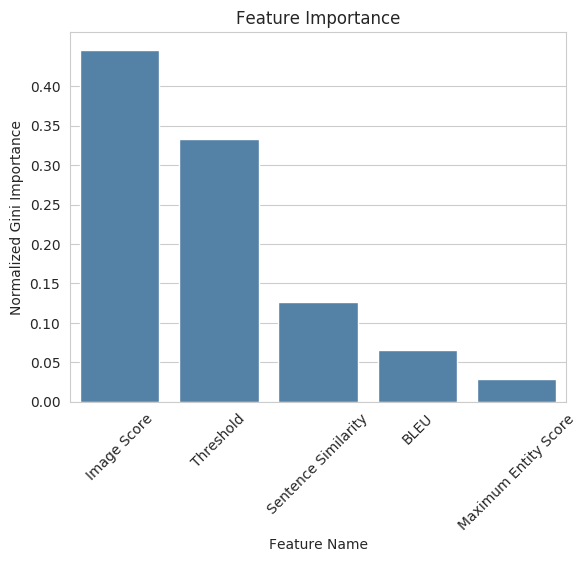
\includegraphics[width=8cm]{FI_old.png}
\caption{Feature Importance in Random Forest Model for predicting if an utterance could be replaced with an image. Image Score is maximum cosine similarity between utterance and images embeddings from CLIP. Threshold is binary feature, indicating if Image Score, Sentence Similarity and Maximum Entity Score is bigger than empirically founded values. Sentence Similarity is cosine distance similarity between utterance embedding and caption embedding, that were generated from corresponding image with VIT-GPT2, where embeddings come from SentenceBert. BLEU is calculated between utterance and generated caption with taking only unigrams into account. Maximum Entity Score is maximum out of Image Scores for each noun in utterance.}
\label{pictorialization::FI}
\end{figure}




\begin{table}[pt]
\caption{Metrics for best (in terms of Precision) Random Forest model for predicting if utterance is replaceable}
\label{TableMetricsRF} 
\begin{center}
\begin{tabular}{lccc}
\hline \bf Metric & Mean & Standart Deviation & Median  \\ \hline
Precision &  0.975000 &  0.156125 &  1.000000 \\
Recall &  0.030990 &  0.006374 &  0.031250 \\
F1 &  0.060042 &  0.012072 &  0.060606 \\
\hline
\end{tabular}
\end{center}
\end{table}


\begin{table}[pt]
\caption{Comparison for different ML Algorithms in terms of Precision and Recall}
\label{TableAlgos} 
\begin{center}
\begin{tabular}{lcc}
\hline \bf Algorithm &  Precision &    Recall \\\hline
Random Forest  &   0.975000 &  0.030990 \\
Kernel SVM &   0.958333 &  0.037500 \\
Gradient Boosting  &   0.816667 &  0.026302 \\
KNN &   0.500188 &  0.035677 \\
\hline
\end{tabular}
\end{center}
\end{table}

